\section{Histograms on the Second Run~\label{sec:sodb9_r2_hist}} 
This section exhibits histograms on the second run of 
INC with its task length increasing from 1 second to 4096 seconds, via EMPv5 without Step 2. 
The detailed description of the base data is from Table~\ref{tab:exp_notes2}.

\begin{table}[h]
\begin{center}
\begin{tabular}{|p{2cm}|p{3cm}|p{3cm}|p{4cm}|p{3.5cm}|} \hline
Machine & Task Length (sec) & Description & Experiment Period & Relevant \linebreak Histograms\\ \hline
{\tt sodb9} (plugged into {\em the upper left} power strip) &  INC1$\sim$INC64 & 1000 samples, each & 2017-03-13 $\sim$ 2017-03-14 & Figs.~\ref{fig:s9_r2_et_hist1},~\ref{fig:s9_r2_et_hist2},~\ref{fig:s9_r2_pt_hist1}, and~\ref{fig:s9_r2_pt_hist2}\\ \hline
%{\tt sodb9} &  INC128$\sim$INC1024 & 300 samples, each & 2017-03-14 $\sim$ 2017-03-21 & 
%Figs.~\ref{fig:s9_r2_et_hist3} and~\ref{fig:s9_r2_pt_hist3}\\ \hline
{\tt sodb9} (plugged into {\em the upper left} power strip) &  INC512$\sim$INC1024 & 300 samples, each & 2017-03-17 $\sim$ 2017-03-21 & 
Figs.~\ref{fig:s9_r2_et_hist3} and~\ref{fig:s9_r2_pt_hist3}\\ \hline
{\tt sodb10} (plugged into {\em the upper left} power strip) & INC2048 & 300 samples & 2017-03-13 $\sim$ 2017-03-20 & Figs.~\ref{fig:inc2048_r2_et_hist_v5} and~\ref{fig:inc2048_r2_hist_v5}\\ \hline
{\tt sodb12} (plugged into {\em the upper right} power strip) & INC4096 & 300 samples & 2017-03-02 $\sim$ 2017-03-17 & Figs.~\ref{fig:inc4096_r2_et_hist_v5} and~\ref{fig:inc4096_r2_hist_v5}\\ \hline
{\tt sodb10} (plugged into {\em the upper left} power strip) & INC8192& 261 samples & 2017-04-27 $\sim$ 2017-05-21 & Figs.~\ref{fig:inc8192_r2_et_hist_v5} and~\ref{fig:inc8192_r2_hist_v5}\\ \hline
{\tt sodb12} (plugged into {\em the upper right} power strip) & INC16384& 130 samples & 2017-04-27 $\sim$ 2017-05-21 & Figs.~\ref{fig:inc16384_r2_et_hist_v5} and~\ref{fig:inc16384_r2_hist_v5}\\ \hline
\end{tabular}
\end{center}
\vspace{-.2in}
\caption{Notes on experiment runs used for histograms\label{tab:exp_notes2}}
\end{table}

INC8192/INC16384 unfortunately stopped in the middle of their runs due to a frozen vnc problem. So couldn't finish 300 samples.

\pagebreak

\subsection{ET}

\begin{figure}[hp!]
	\centering
	\subfigure[ET frequency on INC1 on {\tt sodb9}]{
		\includegraphics[scale=0.43]{repet_data2/1_sec_et_hist_v5.eps}
		\label{fig:inc1_r2_et_hist_v5}
	}
	\subfigure[ET frequency on INC2 on {\tt sodb9}]{
		\includegraphics[scale=0.43]{repet_data2/2_sec_et_hist_v5.eps}
		\label{fig:inc2_r2_et_hist_v5}
	}
	\subfigure[ET frequency on INC4 on {\tt sodb9}]{
		\includegraphics[scale=0.43]{repet_data2/4_sec_et_hist_v5.eps}
		\label{fig:inc4_r2_et_hist_v5}
	}
	\subfigure[ET frequency on INC8 on {\tt sodb9}]{
		\includegraphics[scale=0.43]{repet_data2/8_sec_et_hist_v5.eps}
		\label{fig:inc8_r2_et_hist_v5}
	}
	\caption{ET Histograms of INC1 ... INC8~\label{fig:s9_r2_et_hist1}}
\end{figure}

\begin{figure}[hp!]
	\centering
	\subfigure[ET frequency on INC16 on {\tt sodb9}]{
		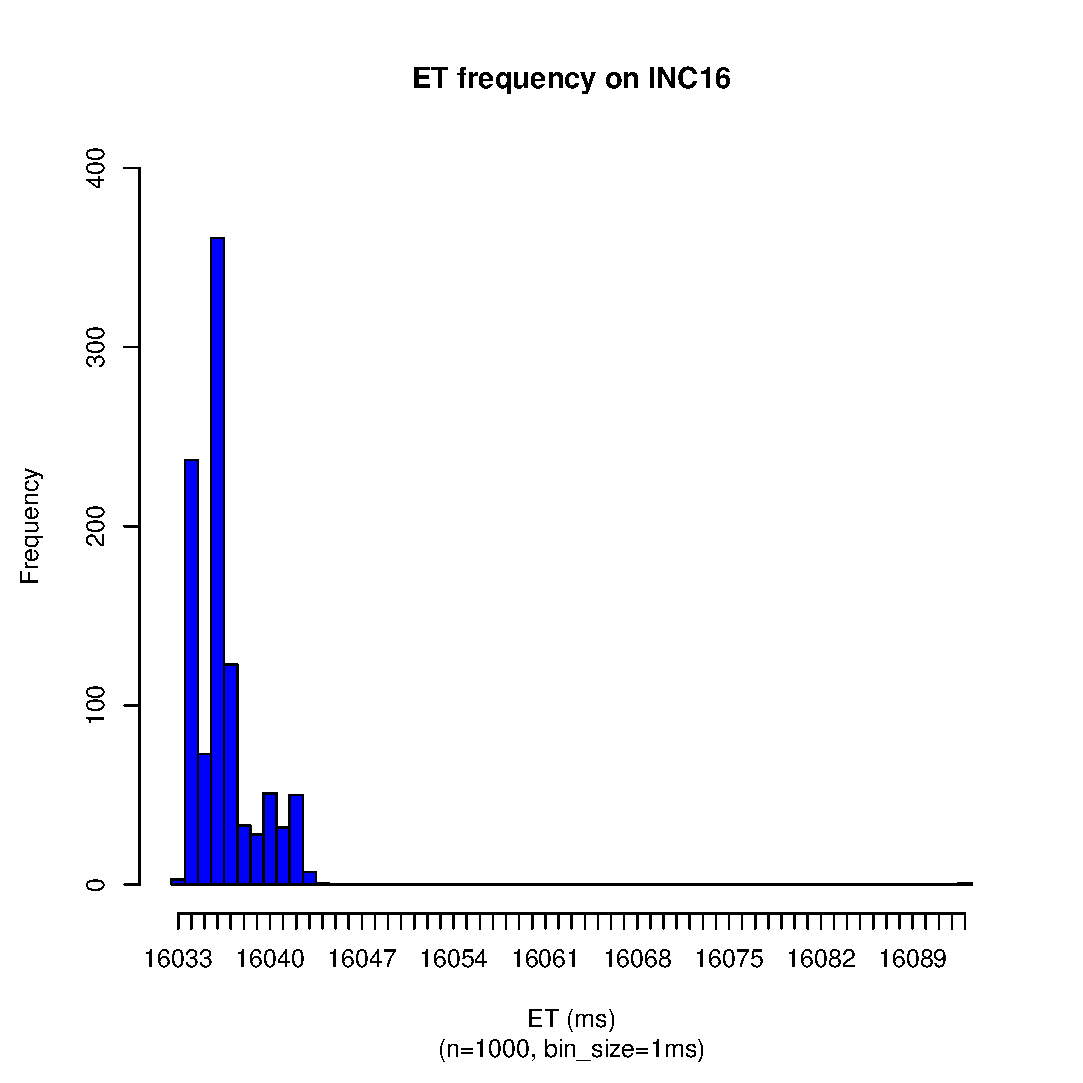
\includegraphics[scale=0.43]{repet_data2/16_sec_et_hist_v5.eps}
		\label{fig:inc16_r2_et_hist_v5}
	}
	\subfigure[ET frequency on INC32 on {\tt sodb9}]{
		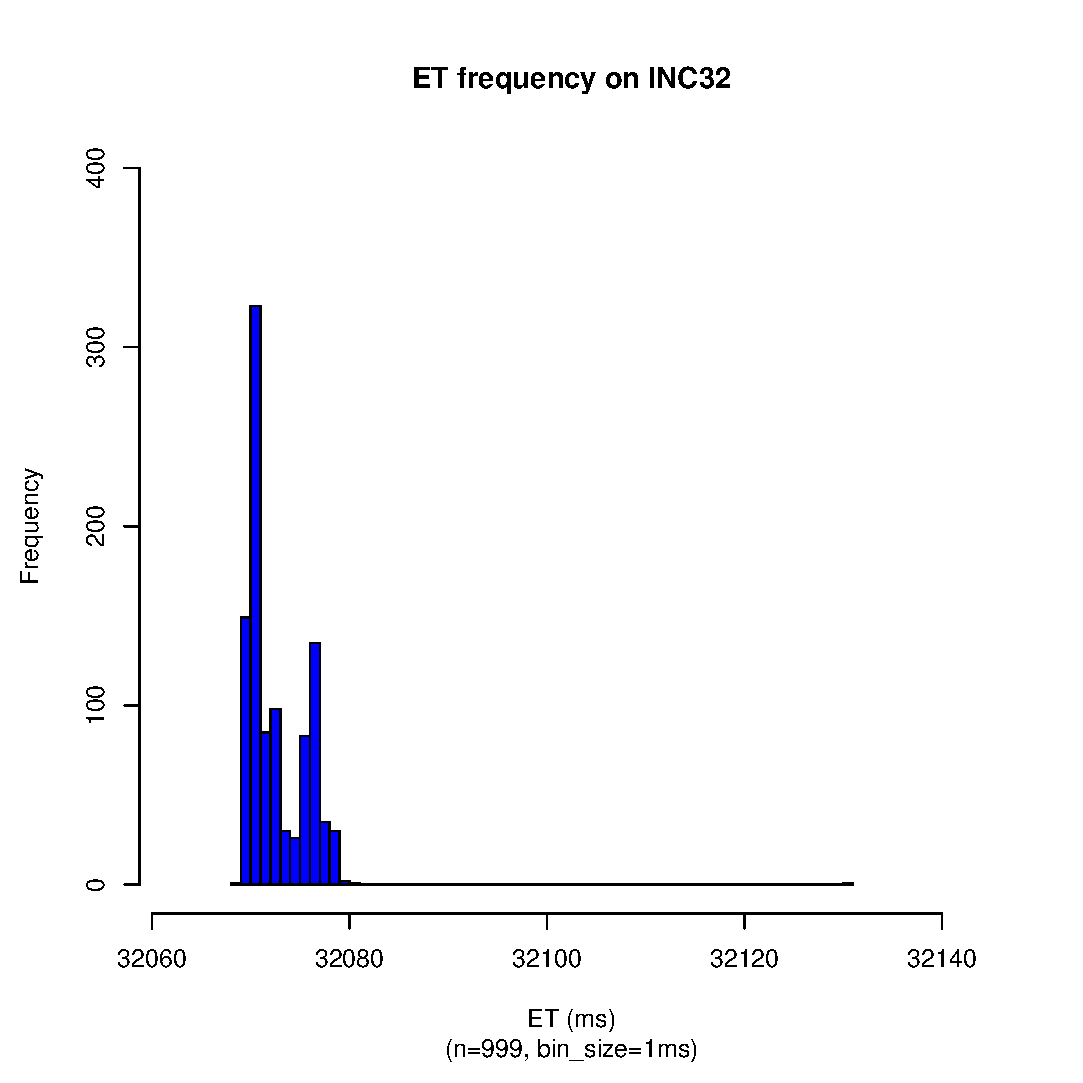
\includegraphics[scale=0.43]{repet_data2/32_sec_et_hist_v5.eps}
		\label{fig:inc32_r2_et_hist_v5}
	}
	\subfigure[ET frequency on INC64 on {\tt sodb9}]{
		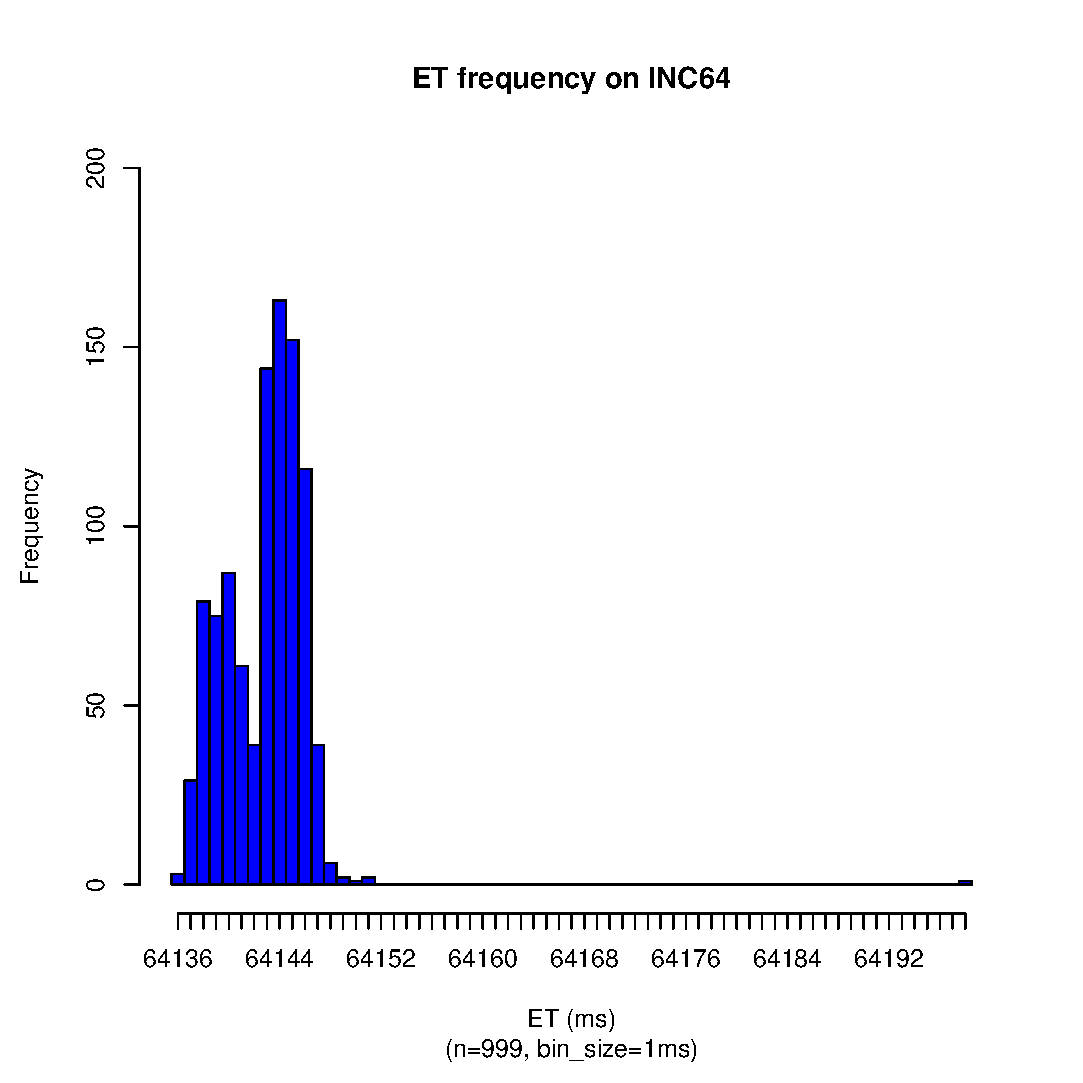
\includegraphics[scale=0.43]{repet_data2/64_sec_et_hist_v5.eps}
		\label{fig:inc64_r2_et_hist_v5}
	}
	\caption{ET Histograms of INC16 ... INC64~\label{fig:s9_r2_et_hist2}}
\end{figure}

\begin{figure}[hp!]
	\centering
	\subfigure[ET frequency on INC128 on {\tt sodb9}]{
		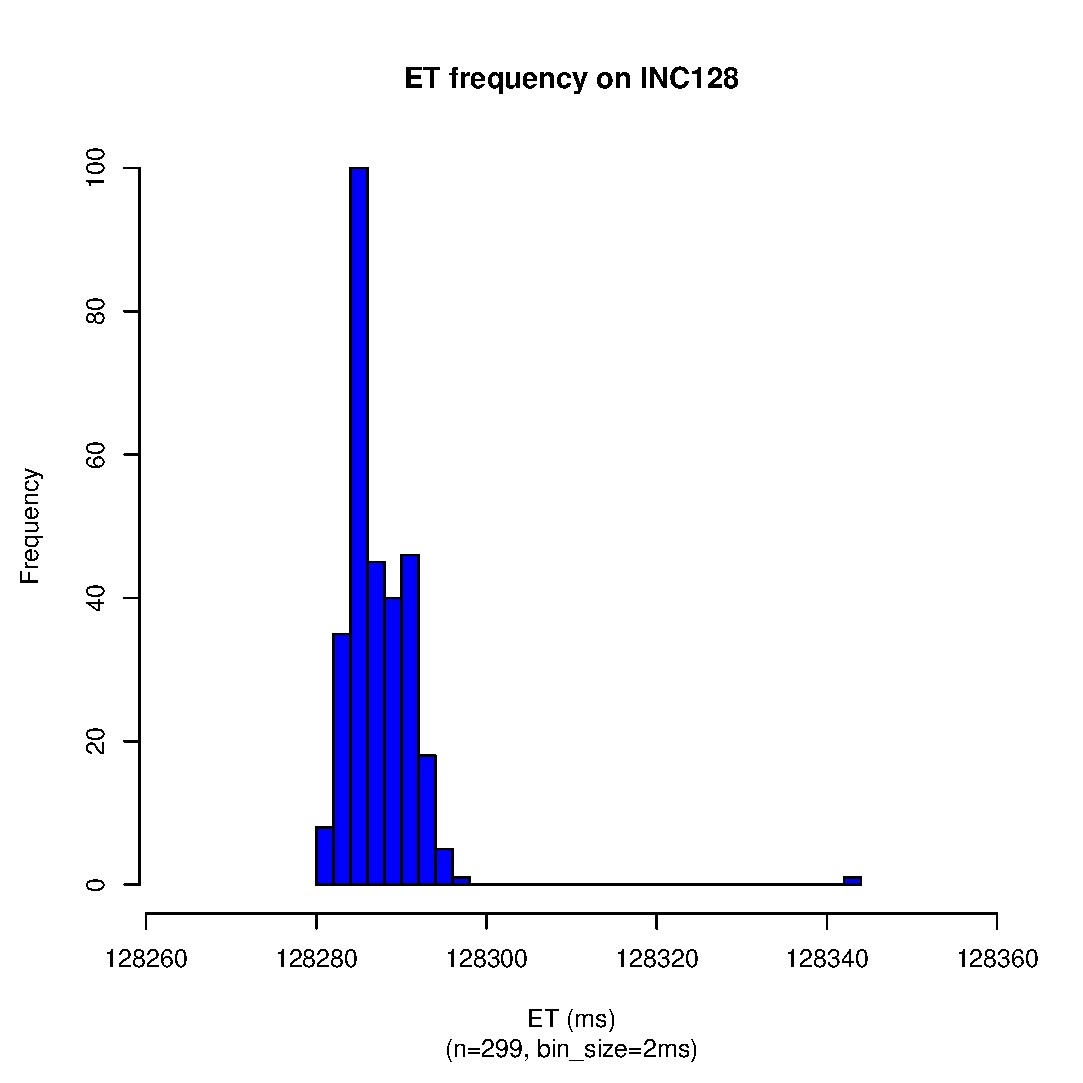
\includegraphics[scale=0.43]{repet_data2/128_sec_et_hist_v5.eps}
		\label{fig:inc128_r2_et_hist_v5}
	}
	\subfigure[ET frequency on INC256 on {\tt sodb9}]{
		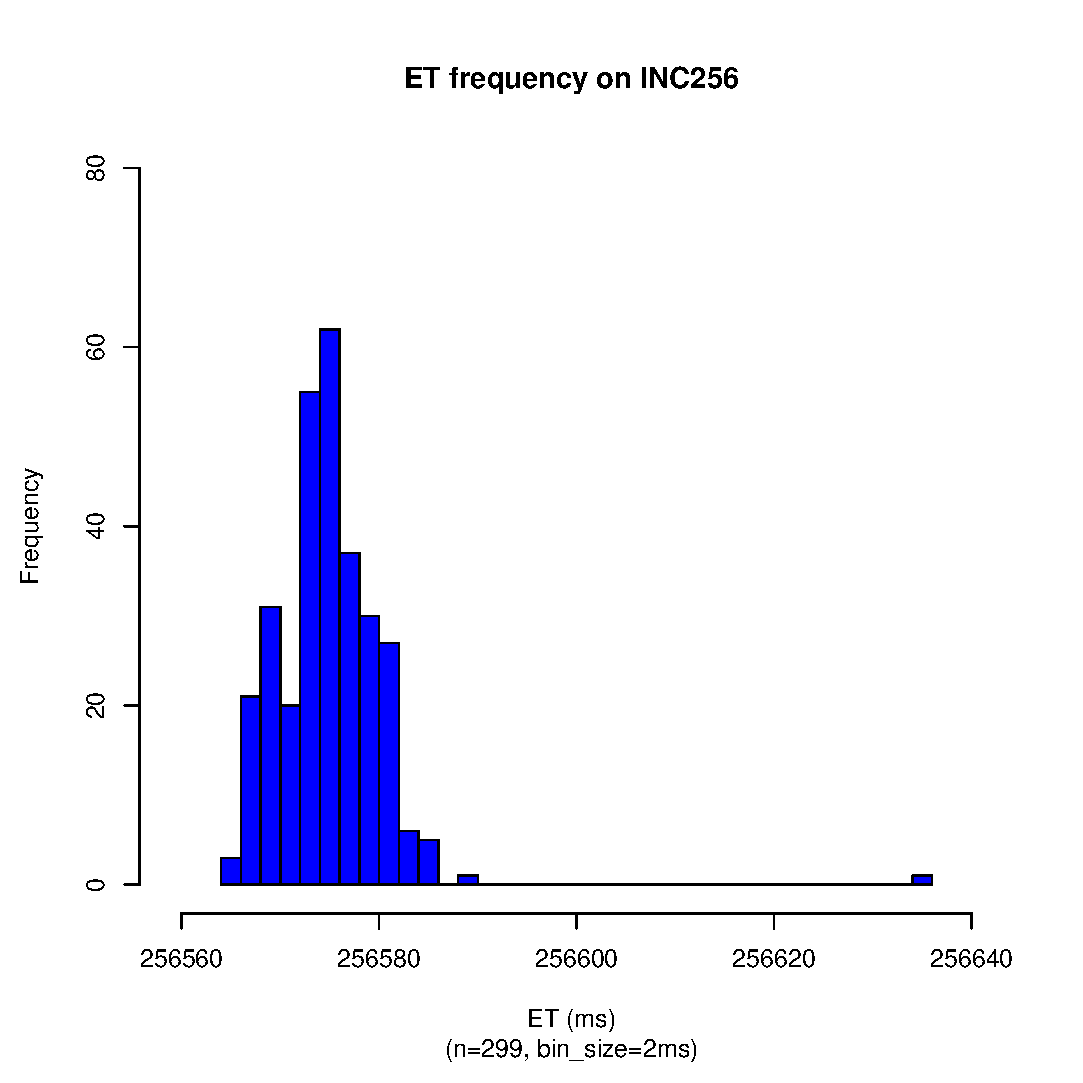
\includegraphics[scale=0.43]{repet_data2/256_sec_et_hist_v5.eps}
		\label{fig:inc256_r2_et_hist_v5}
	}
	\subfigure[ET frequency on INC512 on {\tt sodb9}]{
		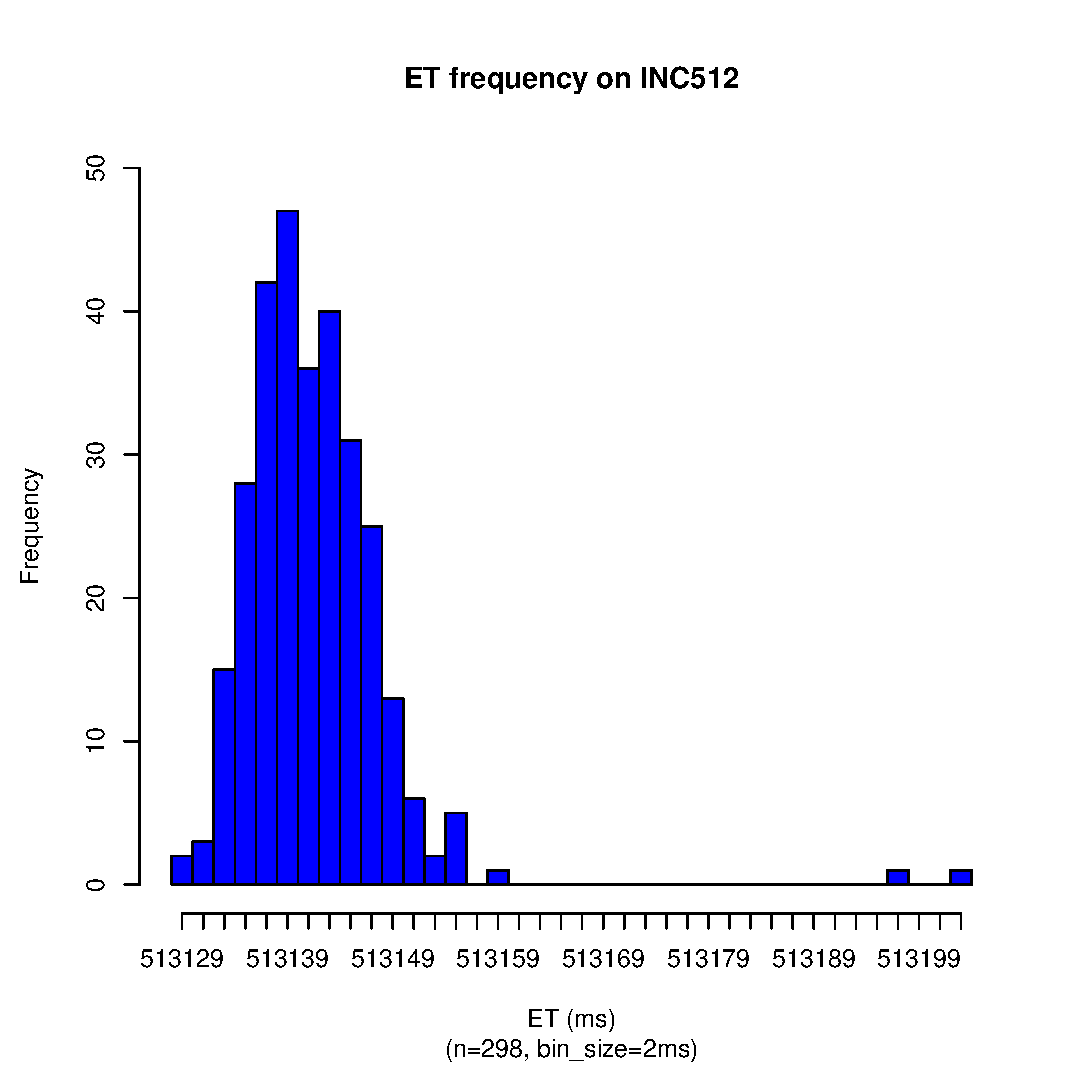
\includegraphics[scale=0.43]{repet_data2/512_sec_et_hist_v5.eps}
		\label{fig:inc512_r2_et_hist_v5}
	}
	\subfigure[ET frequency on INC1024 on {\tt sodb9}]{
		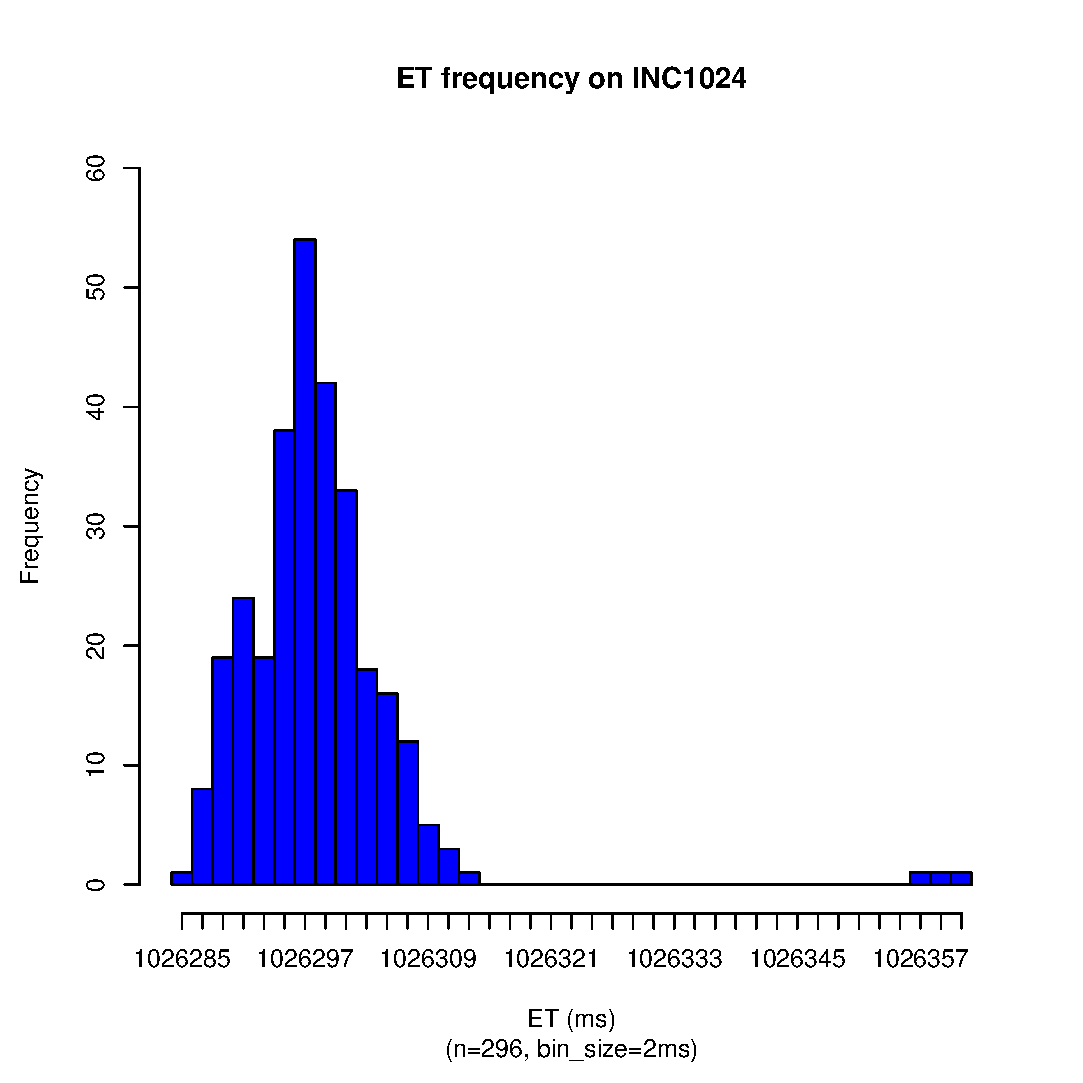
\includegraphics[scale=0.43]{repet_data2/1024_sec_et_hist_v5.eps}
		\label{fig:inc1024_r2_et_hist_v5}
	}
	\caption{ET Histograms of INC128 ... INC1024~\label{fig:s9_r2_et_hist3}}
\end{figure}

\begin{figure}[hp!]
	\centering
	\subfigure[ET frequency on INC2048 on {\tt sodb10}]{
		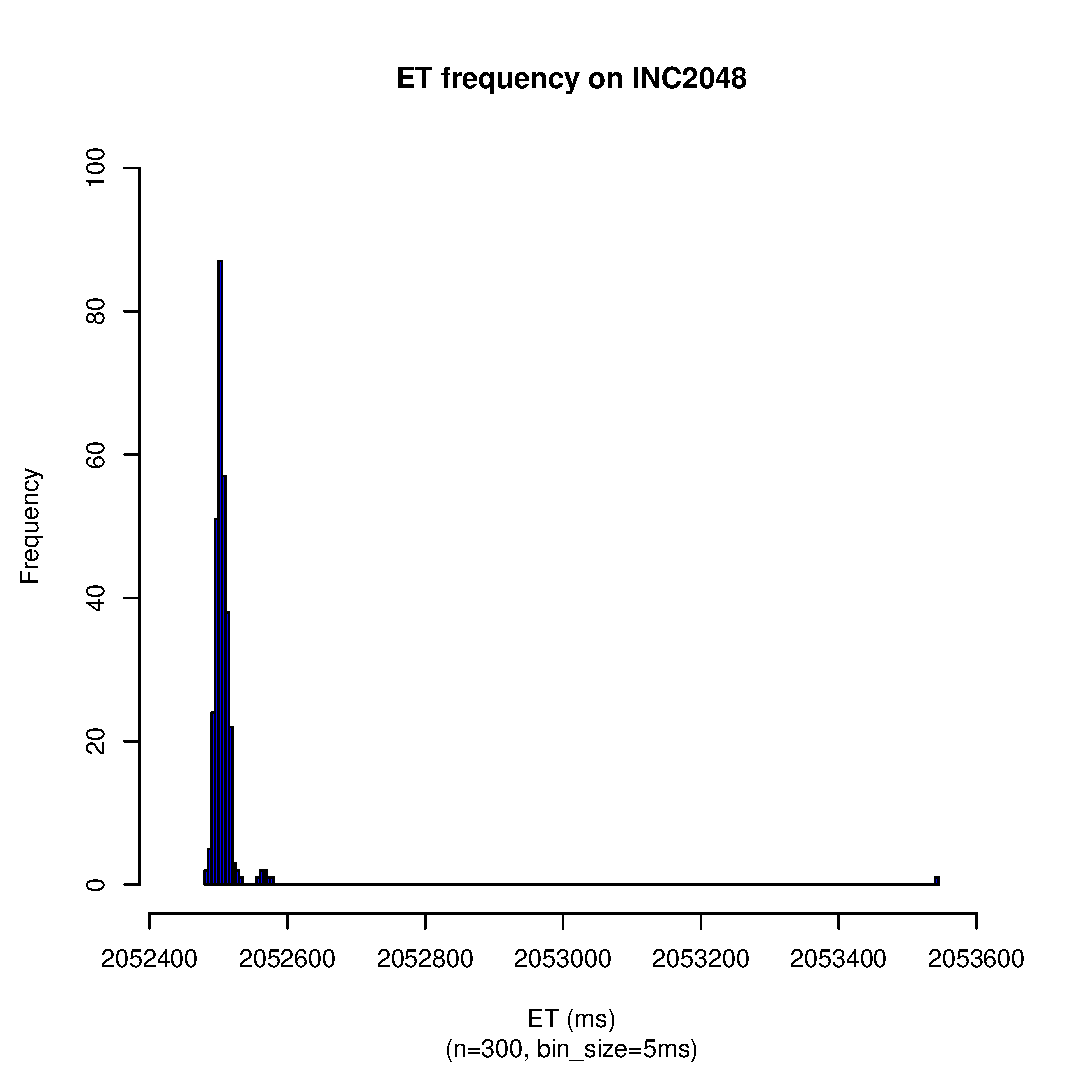
\includegraphics[scale=0.43]{repet_data2/2048_sec_et_hist_v5.eps}
		\label{fig:inc2048_r2_et_hist_v5}
	}
	\subfigure[ET frequency on INC4096 on {\tt sodb12}]{
		\includegraphics[scale=0.43]{repet_data2/4096_sec_et_hist_v5.eps}
		\label{fig:inc4096_r2_et_hist_v5}
	}
	\subfigure[ET frequency on INC8192 on {\tt sodb10}]{
		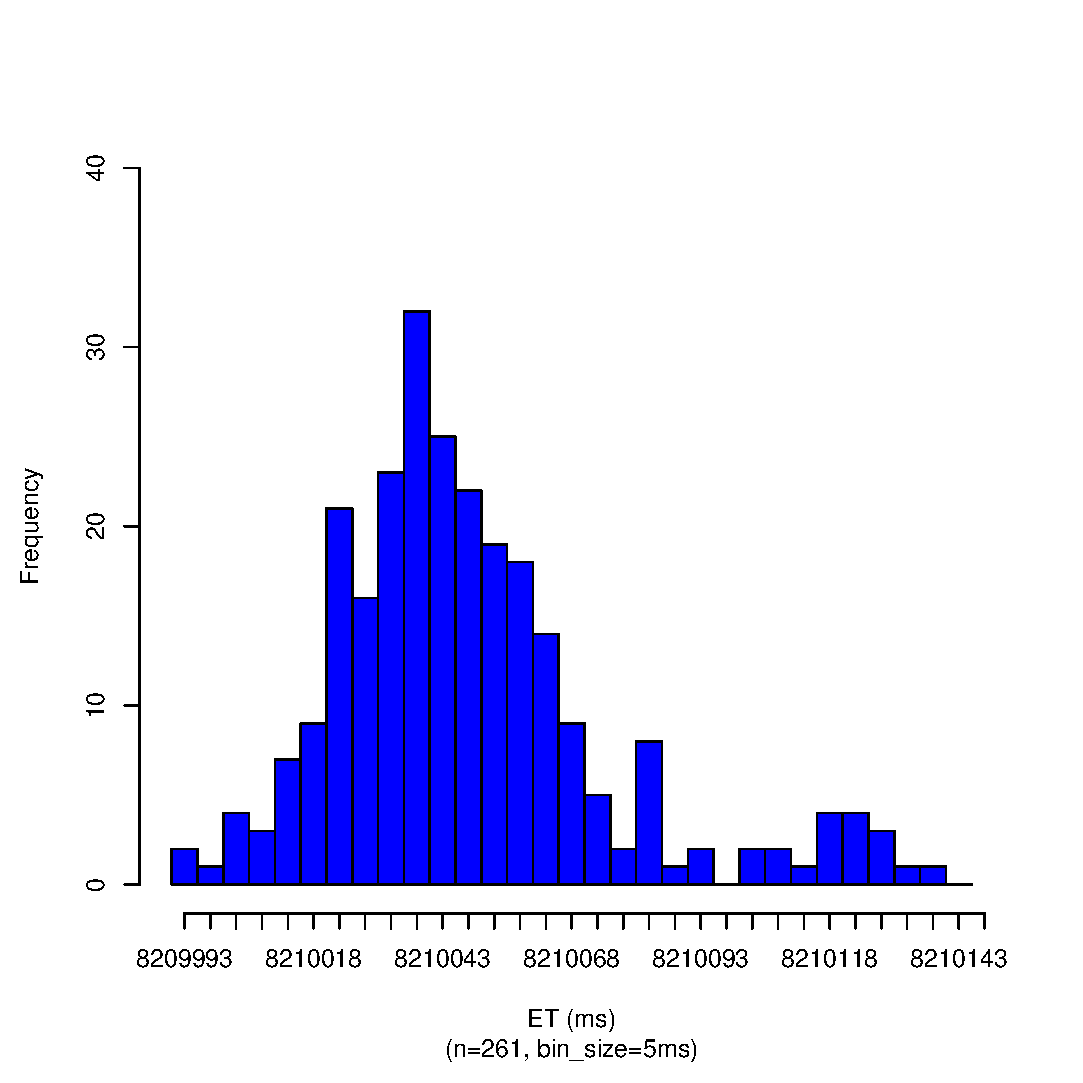
\includegraphics[scale=0.43]{repet_data2/8192_sec_et_hist.eps}
		\label{fig:inc8192_r2_et_hist_v5}
	}
	\subfigure[ET frequency on INC16384 on {\tt sodb12}]{
		\includegraphics[scale=0.43]{repet_data2/16384_sec_et_hist.eps}
		\label{fig:inc16384_r2_et_hist_v5}
	}
	\caption{ET Histograms of INC2048 ... INC16384~\label{fig:s9_r2_et_hist4}}
\end{figure}

\vspace\fill
\clearpage

\subsection{PT}

\begin{figure}[hp!]
	\centering
	\subfigure[PT frequency on INC1 on {\tt sodb9}]{
		\includegraphics[scale=0.43]{repet_data2/1_sec_pt_hist_v5.eps}
		\label{fig:inc1_r2_hist_v5}
	}
	\subfigure[PT frequency on INC2 on {\tt sodb9}]{
		\includegraphics[scale=0.43]{repet_data2/2_sec_pt_hist_v5.eps}
		\label{fig:inc2_r2_hist_v5}
	}
	\subfigure[PT frequency on INC4 on {\tt sodb9}]{
		\includegraphics[scale=0.43]{repet_data2/4_sec_pt_hist_v5.eps}
		\label{fig:inc4_r2_hist_v5}
	}
	\subfigure[PT frequency on INC8 on {\tt sodb9}]{
		\includegraphics[scale=0.43]{repet_data2/8_sec_pt_hist_v5.eps}
		\label{fig:inc8_r2_hist_v5}
	}
	\caption{PT Histograms of INC1 ... INC8~\label{fig:s9_r2_pt_hist1}}
\end{figure}

\begin{figure}[hp!]
	\centering
	\subfigure[PT frequency on INC16 on {\tt sodb9}]{
		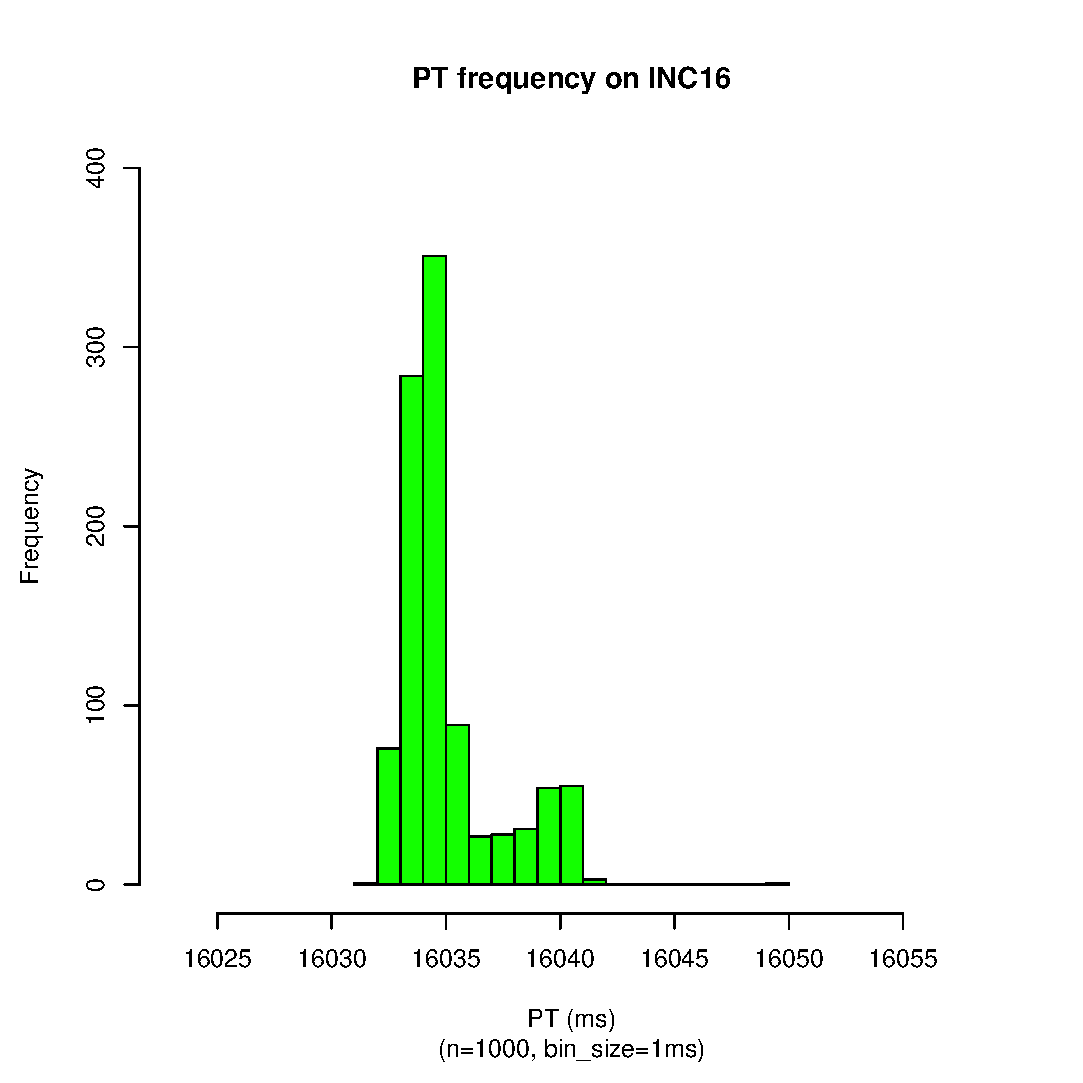
\includegraphics[scale=0.43]{repet_data2/16_sec_pt_hist_v5.eps}
		\label{fig:inc16_r2_hist_v5}
	}
	\subfigure[PT frequency on INC32 on {\tt sodb9}]{
		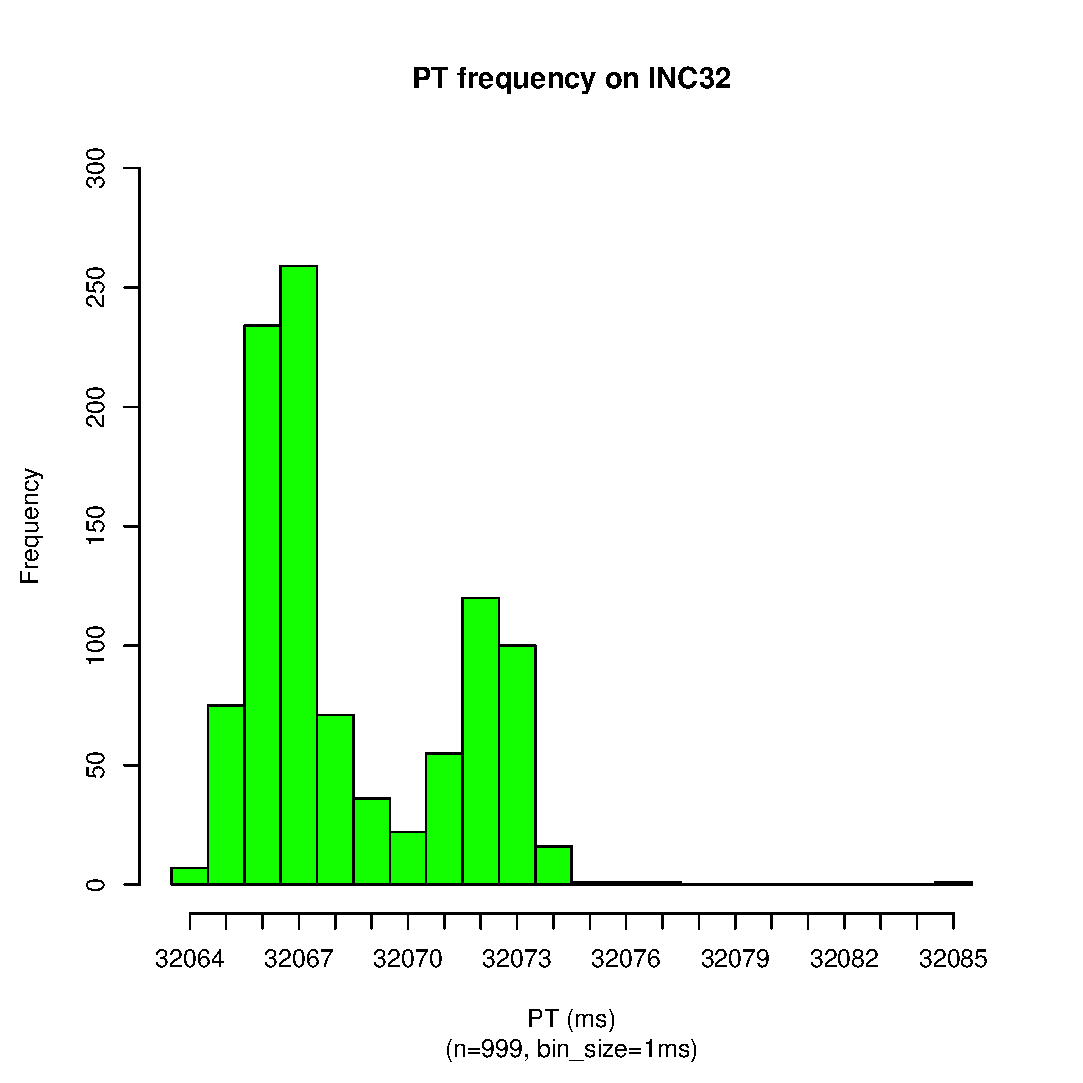
\includegraphics[scale=0.43]{repet_data2/32_sec_pt_hist_v5.eps}
		\label{fig:inc32_r2_hist_v5}
	}
	\subfigure[PT frequency on INC64 on {\tt sodb9}]{
		\includegraphics[scale=0.43]{repet_data2/64_sec_pt_hist_v5.eps}
		\label{fig:inc64_r2_hist_v5}
	}
	\caption{PT Histograms of INC16 ... INC64\label{fig:s9_r2_pt_hist2}}
\end{figure}

\begin{figure}[hp!]
	\centering
	\subfigure[PT frequency on INC128 on {\tt sodb9}]{
		\includegraphics[scale=0.43]{repet_data2/128_sec_pt_hist_v5.eps}
		\label{fig:inc128_r2_hist_v5}
	}
	\subfigure[PT frequency on INC256 on {\tt sodb9}]{
		\includegraphics[scale=0.43]{repet_data2/256_sec_pt_hist_v5.eps}
		\label{fig:inc256_r2_hist_v5}
	}
	\subfigure[PT frequency on INC512 on {\tt sodb9}]{
		\includegraphics[scale=0.43]{repet_data2/512_sec_pt_hist_v5.eps}
		\label{fig:inc512_r2_hist_v5}
	}
	\subfigure[PT frequency on INC1024 on {\tt sodb9}]{
		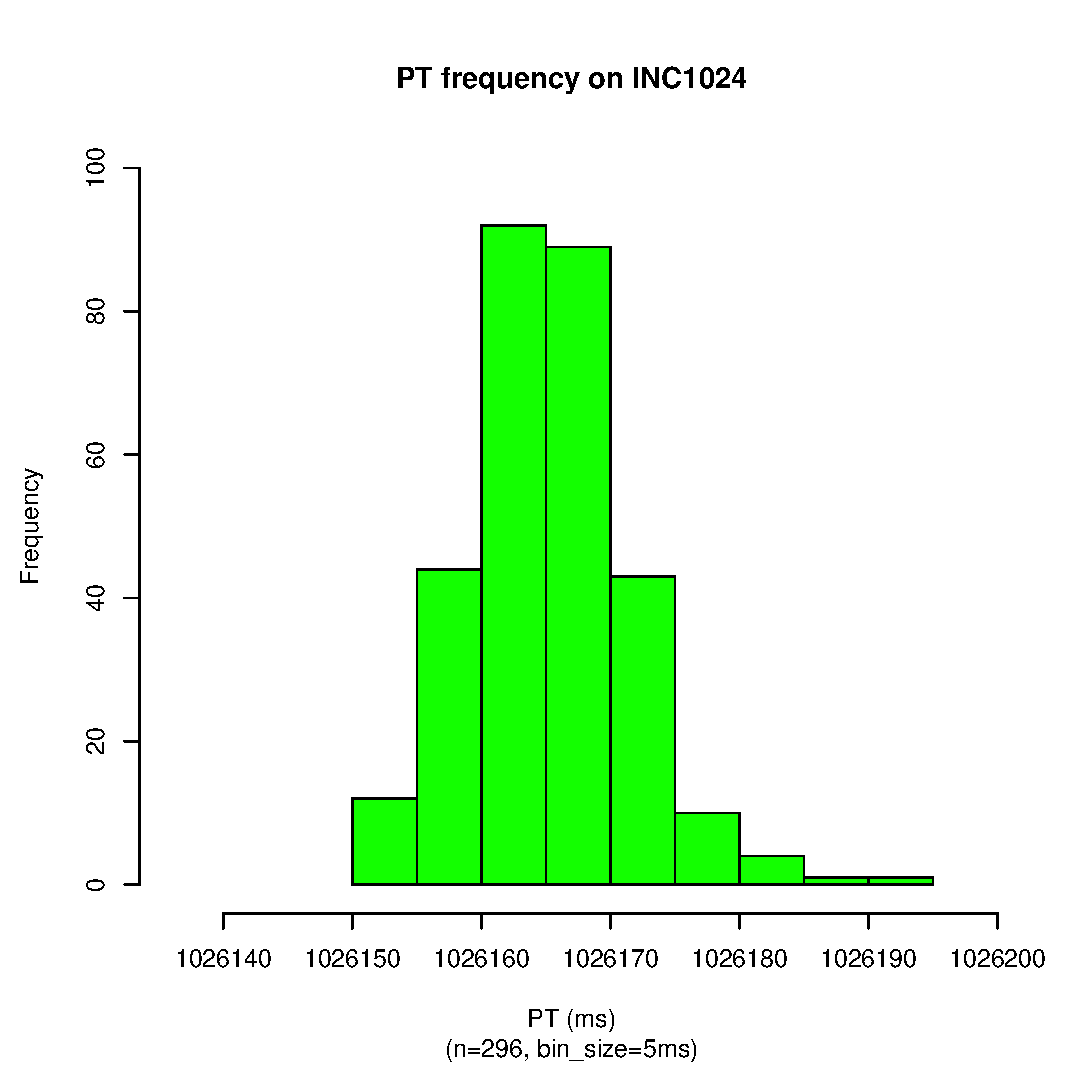
\includegraphics[scale=0.43]{repet_data2/1024_sec_pt_hist_v5.eps}
		\label{fig:inc1024_r2_hist_v5}
	}
	\caption{PT Histograms of INC256 ... INC1024~\label{fig:s9_r2_pt_hist3}}
\end{figure}

\begin{figure}[t]
	\centering
	\subfigure[PT frequency on INC2048 on {\tt sodb10}]{
		\includegraphics[scale=0.43]{repet_data2/2048_sec_pt_hist_v5.eps}
		\label{fig:inc2048_r2_hist_v5}
	}
	\subfigure[PT frequency on INC4096 on {\tt sodb12}]{
		\includegraphics[scale=0.43]{repet_data2/4096_sec_pt_hist_v5.eps}
		\label{fig:inc4096_r2_hist_v5}
	}
	\subfigure[PT frequency on INC8192 on {\tt sodb10}]{
		\includegraphics[scale=0.43]{repet_data2/8192_sec_pt_hist.eps}
		\label{fig:inc8192_r2_hist_v5}
	}
	\subfigure[PT frequency on INC16384 on {\tt sodb12}]{
		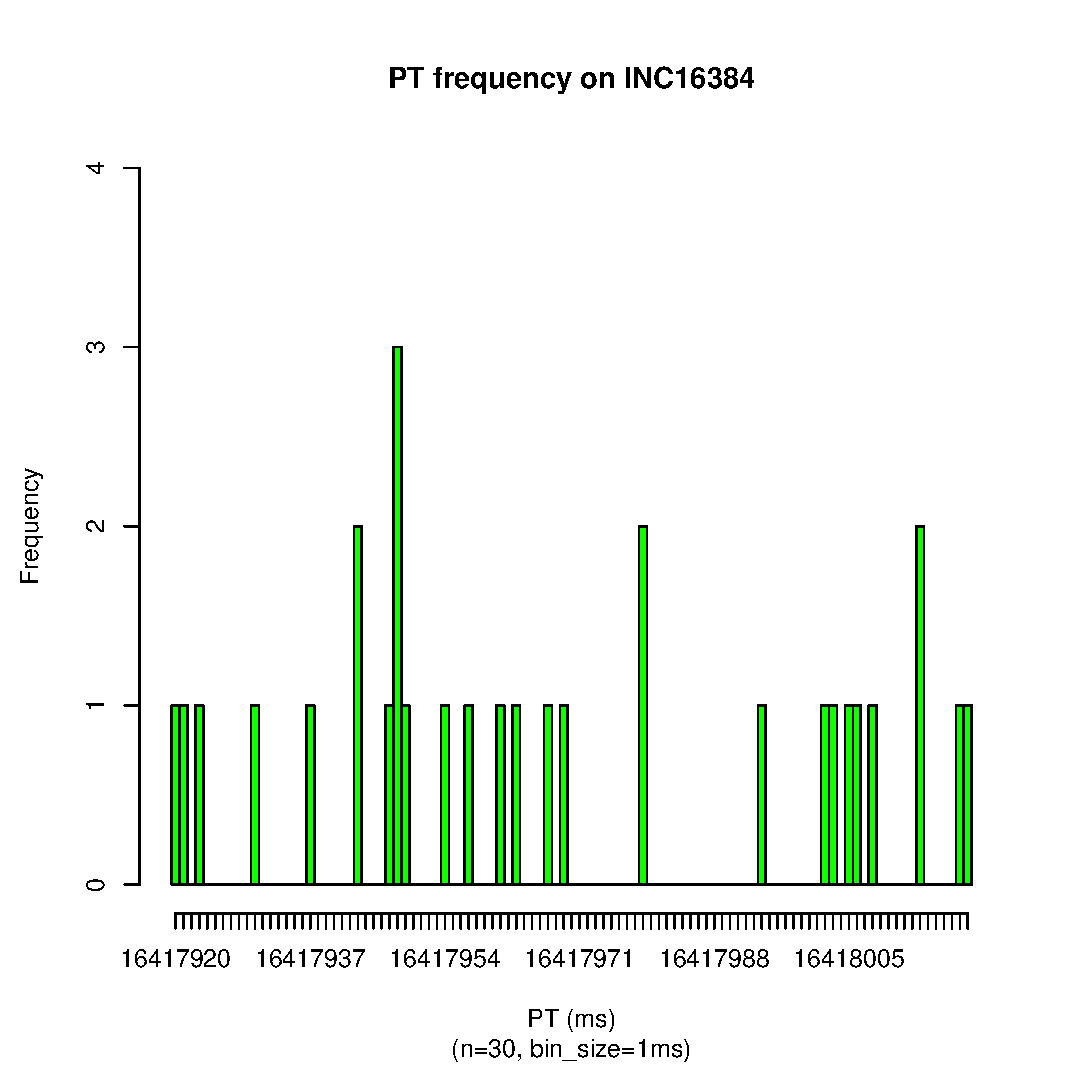
\includegraphics[scale=0.43]{repet_data2/16384_sec_pt_hist.eps}
		\label{fig:inc16384_r2_hist_v5}
	}
	\caption{PT Histograms of INC2048 ... INC16384~\label{fig:s9_r2_pt_hist4}}
\end{figure}

\clearpage
\pagebreak
\subsubsection{Analysis}
In this section we look into what happened inside the peaks observed in a certain histogram. 
We consider Figure~\ref{fig:inc8_r2_hist_v5} for this study. 
In the figure, we see the peaks at 8015 msec, 8020 msec, and 8021 msec. 

Table~\ref{tab:inc8_daemons} shows captured daemons and their runtime statistics per bin 
of figure. Note that bin is at the unit of PT. 
It appears that the peaks are definitely correlated with (1) appearances of some daemons 
and (2) times that those daemons co-ran with INC8. 

\begin{table}[h]
\begin{center}
{\scriptsize
\begin{tabular}{l|l|l|l|l|l|l|l} \hline
TASK\_LEN  & BIN (PT) &  DAEMON   & MIN\_PT  &  MAX\_PT  &  AVG\_PT  &   STD\_PT & Counts \\ \hline
INC8     & 8013  & jbd2/md0-8    & 1     & 1     & 1     & 0     & 1\\ \hline
INC8     & 8013  & kslowd000     & 1     & 1     & 1     & 0     & 1\\ \hline
INC8     & 8013  & md0\_raid1     & 1     & 1     & 1     & 0     & 17\\ \hline
INC8     & 8013  & proc\_monitor  & 196   & 200   & 197.72        & 1.07  & 18\\ \hline \hline

INC8     & 8014  & jbd2/md0-8    & 1     & 1     & 1     & 0     & 5\\ \hline
INC8     & 8014  & kslowd000     & 1     & 1     & 1     & 0     & 35\\ \hline
INC8     & 8014  & kslowd001     & 1     & 1     & 1     & 0     & 26\\ \hline
INC8     & 8014  & md0\_raid1     & 1     & 1     & 1     & 0     & 58\\ \hline
INC8     & 8014  & proc\_monitor  & 196   & 200   & 197.31        & 1.06  & 95\\ \hline \hline

INC8     & {\bf 8015}  & java  & 2     & 7     & 4.5   & 3.54  & 2\\ \hline
INC8     & {\bf 8015}  & jbd2/md0-8    & 1     & 1     & 1     & 0     & 2\\ \hline
INC8     & {\bf 8015}  & kslowd000     & 1     & 1     & 1     & 0     & 86\\ \hline
INC8     & {\bf 8015}  & kslowd001     & 1     & 1     & 1     & 0     & 89\\ \hline
INC8     & {\bf 8015}  & md0\_raid1     & 1     & 1     & 1     & 0     & 18\\ \hline
INC8     & {\bf 8015}  & proc\_monitor  & 196   & 200   & 197.28        & 1.01  & 194\\ \hline\hline

INC8     & 8016  & kslowd000     & 1     & 1     & 1     & 0     & 36\\ \hline
INC8     & 8016  & kslowd001     & 1     & 1     & 1     & 0     & 40\\ \hline
INC8     & 8016  & md0\_raid1     & 1     & 1     & 1     & 0     & 8\\ \hline
INC8     & 8016  & proc\_monitor  & 196   & 200   & 196.45        & .95   & 78\\ \hline\hline

INC8     & 8017  & kslowd000     & 1     & 1     & 1     & 0     & 11\\ \hline
INC8     & 8017  & kslowd001     & 1     & 1     & 1     & 0     & 10\\ \hline
INC8     & 8017  & md0\_raid1     & 1     & 1     & 1     & 0     & 3\\ \hline
INC8     & 8017  & proc\_monitor  & 196   & 200   & 197.15        & 1.16  & 26\\ \hline\hline

INC8     & 8018  & kslowd000     & 1     & 1     & 1     & 0     & 13\\ \hline
INC8     & 8018  & kslowd001     & 1     & 1     & 1     & 0     & 9\\ \hline
INC8     & 8018  & md0\_raid1     & 1     & 1     & 1     & 0     & 6\\ \hline
INC8     & 8018  & proc\_monitor  & 196   & 200   & 197.24        & 1.27  & 29\\ \hline\hline

INC8     & 8019  & jbd2/md0-8    & 1     & 1     & 1     & 0     & 3\\ \hline
INC8     & 8019  & kslowd000     & 1     & 1     & 1     & 0     & 9\\ \hline
INC8     & 8019  & kslowd001     & 1     & 2     & 1.06  & .24   & 18\\ \hline
INC8     & 8019  & md0\_raid1     & 1     & 1     & 1     & 0     & 27\\ \hline
INC8     & 8019  & proc\_monitor  & 196   & 200   & 197.1         & 1.18  & 52\\ \hline\hline

INC8     & {\bf 8020}  & jbd2/md0-8    & 1     & 1     & 1     & 0     & 8\\ \hline
INC8     & {\bf 8020}  & kslowd000     & 1     & 1     & 1     & 0     & 52\\ \hline
INC8     & {\bf 8020}  & kslowd001     & 1     & 1     & 1     & 0     & 57\\ \hline
INC8     & {\bf 8020}  & md0\_raid1     & 1     & 1     & 1     & 0     & 91\\ \hline
INC8     & {\bf 8020}  & proc\_monitor  & 196   & 200   & 197.03        & 1.02  & 180\\ \hline\hline

INC8     & {\bf 8021}  & cifsd         & 1     & 1     & 1     & 0     & 1\\ \hline
INC8     & {\bf 8021}  & java  & 2     & 37    & 19.5  & 24.75         & 2\\ \hline
INC8     & {\bf 8021}  & kslowd000     & 1     & 1     & 1     & 0     & 146\\ \hline
INC8     & {\bf 8021}  & kslowd001     & 1     & 1     & 1     & 0     & 143\\ \hline
INC8     & {\bf 8021}  & md0\_raid1     & 1     & 1     & 1     & 0     & 11\\ \hline
INC8     & {\bf 8021}  & proc\_monitor  & 196   & 198   & 197.15        & .98   & 299\\ \hline\hline

INC8     & 8022  & kslowd000     & 1     & 1     & 1     & 0     & 20\\ \hline
INC8     & 8022  & kslowd001     & 1     & 1     & 1     & 0     & 9\\ \hline
INC8     & 8022  & proc\_monitor  & 196   & 198   & 196.07        & .37   & 29\\ \hline\hline
\end{tabular}
}
\end{center}
\caption{Daemons observed from the INC8 run~\label{tab:inc8_daemons}}
\end{table}

\clearpage
\newpage

\subsubsection{Analysis on Some Outliers Found from INC16 and INC64 on {\tt sodb9}}
In this section we investigate what happened about some outlying samples on INC16 and INC64 
shown in Figures~\ref{fig:inc16_r2_hist_v5} and~\ref{fig:inc64_r2_hist_v5}.

%Regarding INC16, we looked into detailed information of processes that were 
%captured at some executions corresponding to the two bins of 16,041 (frequency = 3) 
%and 16,050 (frequency = 1) msecs in PT. 
Regarding INC16, we looked into detailed information of processes that were 
captured at one execution corresponding to the bin of 16,050 (frequency = 1) msec in PT. 
For the purpose of comparison, we also explored processes captured 
at the second-highest bin of 16,041 msec in PT. 

Table~\ref{tab:inc16_daemons} shows the overall information of the captured processes at the two bins. 
As indicated by the table, there were 
some infrequent daemon processes such as {\tt sshd}, {\tt grep}, {\tt md0\_raid1}, {\tt cifsd}, running for some time 
when the INC16 program was run.

\begin{table}[h]
\begin{center}
\begin{tabular}{|l|l|l|l|} \hline
Iteration number &  Process ID & Process Name  & PT (in msec)\\ \hline
77 (, 209, or 569) & 10185 & {\tt incr\_work} (=INC16) & 16,041 \\ \hline
& 28525 & {\tt proc\_monitor} & 196 \\ \hline
& 167 & {\tt kslowd001} &  1 \\ \hline
& 166 & {\tt kslowd000} &  1 \\ \hline \hline 
703 & 10185 & {\tt incr\_work} (=INC16) & 16,050 \\ \hline
& 28525 & {\tt proc\_monitor} & 196 \\ \hline
& 12322 & {\tt sshd} & 14 \\ \hline
& 12313 & {\tt sshd}  & 13 \\ \hline
& 12324 & {\tt grep}  &  6 \\ \hline
& 472 & {\tt md0\_raid1} &  2 \\ \hline
& 12314 & {\tt sshd}  &  2 \\ \hline
& 12315 & {\tt grep}  &  2 \\ \hline
& 12319 & {\tt grep}  &  1 \\ \hline
& 167 & {\tt kslowd001} &  1 \\ \hline
& 12323 & {\tt sshd}  &  1 \\ \hline
& 166 & {\tt kslowd000} &  1 \\ \hline
& 12328 & {\tt grep}  &  1 \\ \hline
& 1925 & {\tt cifsd} &  1 \\ \hline 
\hline
\end{tabular}
\end{center}
\caption{Daemons observed at the second-rightmost and rightmost bins in Figure~\ref{fig:inc16_r2_hist_v5}~\label{tab:inc16_daemons}}
\end{table}

Regarding INC64, we looked into detailed information of processes that were 
captured at one execution corresponding to the bin of 64,151 (frequency = 1) msec in PT. 
For the purpose of comparison, we also explored processes captured 
at the second-highest bin of 16,041 msec in PT. 

Table~\ref{tab:inc64_daemons} shows the overall information of the captured processes at the two bins. 
As indicated by the table, there were also 
the same kind of infrequent daemon processes such as {\tt sshd}, {\tt grep}, {\tt md0\_raid1} as well as 
{\tt java} running for some time when the INC64 program was run. 
%In particular, we may not able to avoid hosting java for the longer INCs 
%as it appears by all means java ran due to any reason including GC 
%during such INCs' execution for some time. 
It is conjectured that for a longer INC program, it is more frequent to have {\tt java} with some positive time in PT. 

\begin{table}[h]
\begin{center}
\begin{tabular}{|l|l|l|l|} \hline
Iteration number &  Process ID & Process Name  & PT (in msec)\\ \hline
795 (, 125, or 236) & 16256 & {\tt incr\_work} (=INC64) & 16,142 \\ \hline
	& 28525 & {\tt proc\_monitor} & 198 \\ \hline
	& 167 & {\tt kslowd001} &  4 \\ \hline
	& 166 & {\tt kslowd000} &  3 \\ \hline 
(125) & (472) & ({\tt md0\_raid1}) & (2) \\ \hline
    & 16246 & {\tt java} &  2 \\ \hline 
\hline 
759 & 16256 & {\tt incr\_work} (=INC64) & 64,151 \\ \hline
& 28525 & {\tt proc\_monitor} & 198 \\ \hline
& 19320 & {\tt sshd} & 13 \\ \hline
& 19329 & {\tt sshd}  & 12 \\ \hline
& 19331 & {\tt grep}  &  5 \\ \hline
& 19322 & {\tt grep}  &  5 \\ \hline
& 167 & {\tt kslowd001} & 3\\ \hline
& 166 & {\tt kslowd000} &  3 \\ \hline
& 16246 & {\tt java} &  2 \\ \hline
& 2067 & {\tt sshd}  &  2 \\ \hline
& 19335 & {\tt grep}  &  1 \\ \hline
& 19330 & {\tt sshd}  &  1 \\ \hline
& 472 & {\tt md0\_raid1} &  1 \\ \hline
& 19326 & {\tt grep}  &  1 \\ \hline
\hline
\end{tabular}
\end{center}
\caption{Daemons observed at the second-rightmost and rightmost bins in Figure~\ref{fig:inc64_r2_hist_v5}~\label{tab:inc64_daemons}}
\end{table}

\clearpage
\newpage
